\documentclass[../main.tex]{subfiles}

\begin{document}
\chapter{Roots: Open Methods}
\label{chap:chap6}

\begin{center}
    \Large{\textbf{CHAPTER OBJECTIVES}}
\end{center}
The primary objective of this chapter is to acquaint you with open methods for finding
the root of a single nonlinear equation. Specific objectives and topics covered are

\begin{itemize}
    \item Recognizing the difference between bracketing and open methods for root
    location.
    \item Understanding the fixed-point iteration method and how you can evaluate its
    convergence characteristics.
    \item Knowing how to solve a roots problem with the Newton-Raphson method and
    appreciating the concept of quadratic convergence.
    \item Knowing how to implement both the secant and the modified secant methods.
    \item Understanding how Brent's method combines reliable bracketing methods with
    fast open methods to locate roots in a robust and efficient manner.
    \item Knowing how to use MATLAB's \texttt{fzero} function to estimate roots.
    \item Learning how to manipulate and determine the roots of polynomials with
    MATLAB.
\end{itemize}

\noindent For the bracketing methods in Chap. 5, the root is located within an interval prescribed
by a lower and an upper bound. Repeated application of these methods always results
in closer estimates of the true value of the root. Such methods are said to be \emph{convergent}
because they move closer to the truth as the computation progresses (Fig. 6.1a).

In contrast, the \emph{open methods} described in this chapter require only a single starting
value or two starting values that do not necessarily bracket the root. As such, they sometimes
\emph{diverge} or move away from the true root as the computation progresses (Fig. 6.1b).
However, when the open methods converge (Fig. 6.1c) they usually do so much more
quickly than the bracketing methods. We will begin our discussion of open techniques with
a simple approach that is useful for illustrating their general form and also for demonstrating
the concept of convergence.\\

\begin{figure}[h]
    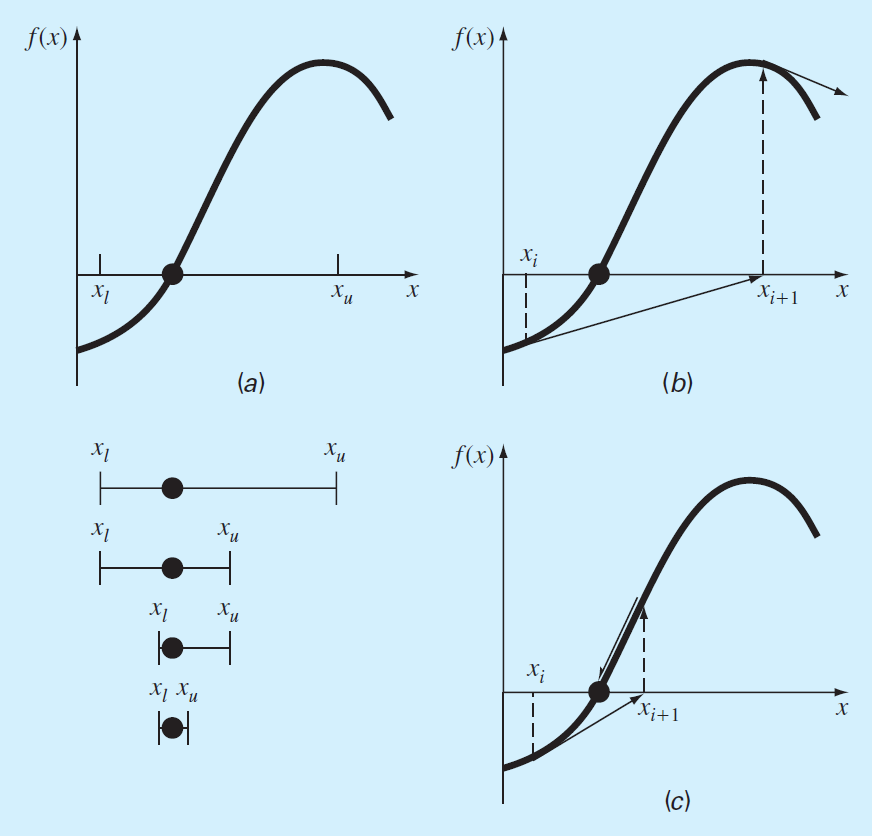
\includegraphics[width = 0.5\linewidth]{./images/fig_6_1}
    \caption{Graphical depiction of the fundamental difference between the (a) bracketing and (b) and (c)
    open methods for root location. In (a), which is bisection, the root is constrained within the interval
    prescribed by $x_l$ and $x_u$ . In contrast, for the open method depicted in (b) and (c), which is
    Newton-Raphson, a formula is used to project from $x_i$ to $x_i+1$ in an iterative fashion. Thus the
    method can either (b) diverge or (c) converge rapidly, depending on the shape of the function
    and the value of the initial guess.}
\end{figure}
\bigskip

\section[SIMPLE FIXED-POINT ITERATION]{SIMPLE FIXED-POINT ITERATION}
\noindent As just mentioned, open methods employ a formula to predict the root. Such a formula can
be developed for simple \emph{fixed-point iteration} (or, as it is also called, \emph{one-point iteration} or
\emph{successive substitution}) by rearranging the function $f (x) = 0$ so that $x$ is on the left-hand
side of the equation:

$x = g(x)$
\hfill (6.1)\\

\noindent This transformation can be accomplished either by algebraic manipulation or by simply
adding $x$ to both sides of the original equation.

The utility of Eq. (6.1) is that it provides a formula to predict a new value of $x$ as a
function of an old value of $x$. Thus, given an initial guess at the root $x_i$ , Eq. (6.1) can be
used to compute a new estimate $x_{i+1}$ as expressed by the iterative formula\\

$x_{i+1} = g(x_i)$
\hfill (6.2)\\

\noindent As with many other iterative formulas in this book, the approximate error for this equation
can be determined using the error estimator:\\

$\epsilon_a = \left\lvert \dfrac{x_{i+1}-x_i}{x_{i+1}} \right\rvert 100\%$
\hfill (6.3)\\

\begin{example} Simple Fixed-Point Iteration\\
    
    \noindent\textbf{Problem Statement.}\quad Use simple fixed-point iteration to locate the root of
    $f(x) = e^{-x}-x$\\

    \noindent\textbf{Solution.} The function can be separated directly and expressed in the form of Eq. (6.2) as\\

    $x_{i+1} = e^{-x_i}$\\

    \noindent Starting with an initial guess of $x_0 = 0$, this iterative equation can be applied to compute:\\

    \begin{figure}[h]
        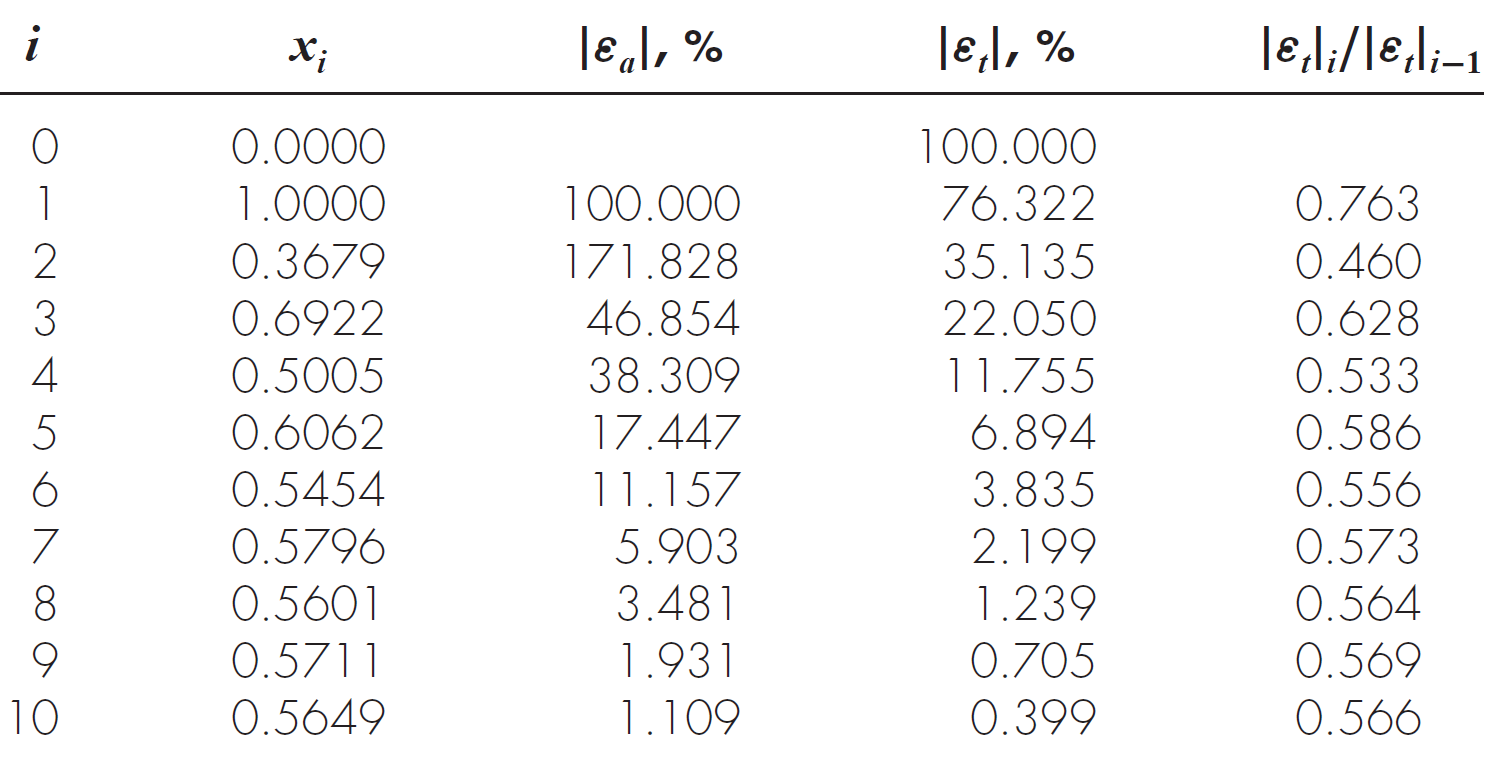
\includegraphics[width=0.6\linewidth]{./images/example_6_1_1}
    \end{figure}

    \noindent Thus, each iteration brings the estimate closer to the true value of the root: 0.56714329.
\end{example}

Notice that the true percent relative error for each iteration of Example 6.1 is roughly
proportional (for this case, by a factor of about 0.5 to 0.6) to the error from the previous
iteration. This property, called \emph{linear convergence}, is characteristic of fixed-point iteration.

Aside from the ``rate'' of convergence, we must comment at this point about the ``possibility'' 
of convergence. The concepts of convergence and divergence can be depicted
graphically. Recall that in Section 5.2, we graphed a function to visualize its structure and
behavior. Such an approach is employed in Fig. 6.2a for the function $f (x) = e^{-x} - x$ . An
alternative graphical approach is to separate the equation into two component parts, as in\\

$f_1(x)=f_2(x)$\\

\noindent Then the two equations\\

$y_1 = f_1(x)$
\hfill (6.4)\\

\noindent and\\

$y_2=f_2(x)$
\hfill (6.5)\\

\noindent can be plotted separately (Fig. 6.2b). The $x$ values corresponding to the intersections of
these functions represent the roots of $f (x) = 0$.

\begin{figure}[h]
    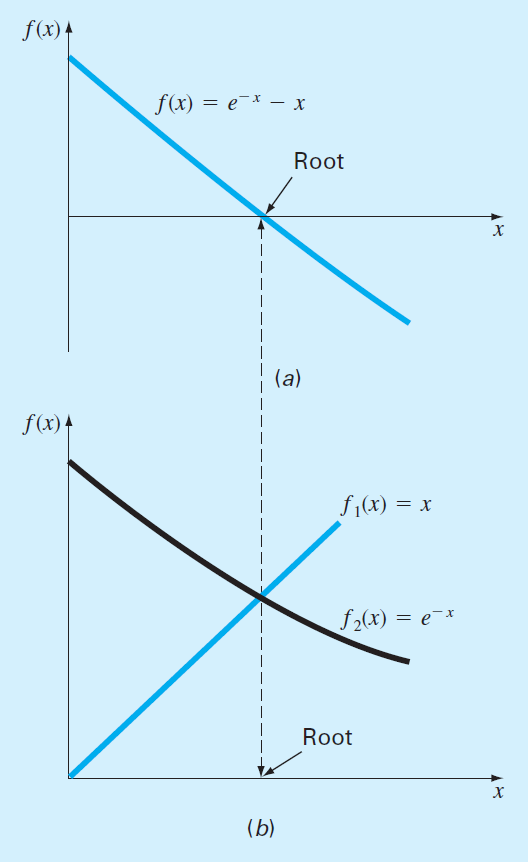
\includegraphics[width=0.4\linewidth]{./images/fig_6_2}
    \caption{Two alternative graphical methods for determining the root of $f (x) = e^{-x} - x$. (a) Root at the
    point where it crosses the x axis; (b) root at the intersection of the component functions.}
\end{figure}

The two-curve method can now be used to illustrate the convergence and divergence
of fixed-point iteration. First, Eq. (6.1) can be reexpressed as a pair of equations $y_1 = x$
and $y_2 = g(x)$. These two equations can then be plotted separately. As was the case with
Eqs. (6.4) and (6.5), the roots of $f (x) = 0$ correspond to the abscissa value at the intersection
of the two curves. The function $y_1 = x$ and four different shapes for $y_2 = g(x)$ are
plotted in Fig. 6.3.

For the first case (Fig. 6.3a), the initial guess of $x_0$ is used to determine the corresponding
point on the $y_2$ curve $[x_0, g(x_0)]$. The point $[x_1, x_1]$ is located by moving left horizontally to
the $y_1$ curve. These movements are equivalent to the first iteration of the fixed-point method:\\

$x_1 = g(x_0)$\\

\noindent Thus, in both the equation and in the plot, a starting value of $x_0$ is used to obtain an estimate
of $x_1$. The next iteration consists of moving to $[x_1, g(x_1)]$ and then to $[x_2, x_2]$. This
iteration is equivalent to the equation\\

$x_2 = g(x_1)$\\

\begin{figure}[h]
    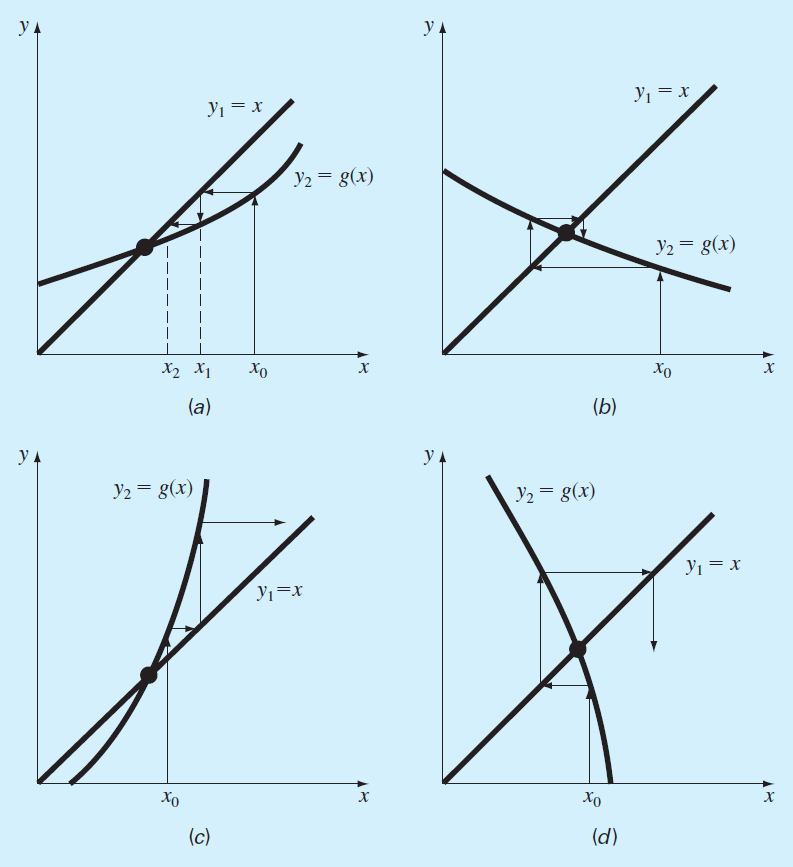
\includegraphics[width=0.65\linewidth]{./images/fig_6_3}
    \caption{Graphical depiction of (a) and (b) convergence and (c) and (d) divergence of simple fixed-point
    iteration. Graphs (a) and (c) are called monotone patterns whereas (b) and (c) are called
    oscillating or spiral patterns. Note that convergence occurs when $\left\lvert g'(x) \right\rvert < 1$ }
\end{figure}

The solution in Fig. 6.3a is \emph{convergent} because the estimates of $x$ move closer to the
root with each iteration. The same is true for Fig. 6.3b. However, this is not the case for
Fig. 6.3c and d, where the iterations diverge from the root.

A theoretical derivation can be used to gain insight into the process. As described in
Chapra and Canale (2010), it can be shown that the error for any iteration is linearly proportional
to the error from the previous iteration multiplied by the absolute value of the
slope of $g$:\\

$E_{i+1} = g'(\xi)E_i$\\

\noindent Consequently, if $\left\lvert g' \right\rvert < 1$, the errors decrease with each iteration. For $\left\lvert g' \right\rvert > 1$ the errors
grow. Notice also that if the derivative is positive, the errors will be positive, and hence the
errors will have the same sign (Fig. 6.3a and c). If the derivative is negative, the errors will
change sign on each iteration (Fig. 6.3b and d).\\
\bigskip

\section[NEWTON-RAPHSON]{NEWTON-RAPHSON}
\noindent Perhaps the most widely used of all root-locating formulas is the \emph{Newton-Raphson method}
(Fig. 6.4). If the initial guess at the root is $x_i$, a tangent can be extended from the point
$[x_i , f (x_i )]$. The point where this tangent crosses the $x$ axis usually represents an improved
estimate of the root.

The Newton-Raphson method can be derived on the basis of this geometrical interpretation.
As in Fig. 6.4, the first derivative at $x$ is equivalent to the slope:\\

$f'(x_i) = \dfrac{f(x_i)-0}{x_i-x_{i+1}}$\\

\noindent which can be rearranged to yield\\

$x_{i+1} = x_i - \dfrac{f(x_i)}{f'(x_i)}$
\hfill (6.6)\\

\noindent which is called the \emph{Newton-Raphson formula.}\\

\begin{example} Newton-Raphson Method\\

    \noindent\textbf{Problem Statement}\quad Use the Newton-Raphson method to estimate the root of $f (x) =e^{-x} - x$
     employing an initial guess of $x_0 = 0$.\\

    \noindent\textbf{Solution.}\quad The first derivative of the function can be evaluated as\\

     $f'(x) = -e^{-x}-1$\\

    \noindent which can be substituted along with the original function into Eq. (6.6) to give\\

    $x_{i+1}= x_i-\dfrac{e^{-x_i}-x_i}{-e^{-x_i}-1}$\\

    \noindent Starting with an initial guess of $x_0 = 0$, this iterative equation can be applied to compute

    \begin{figure}[h]
        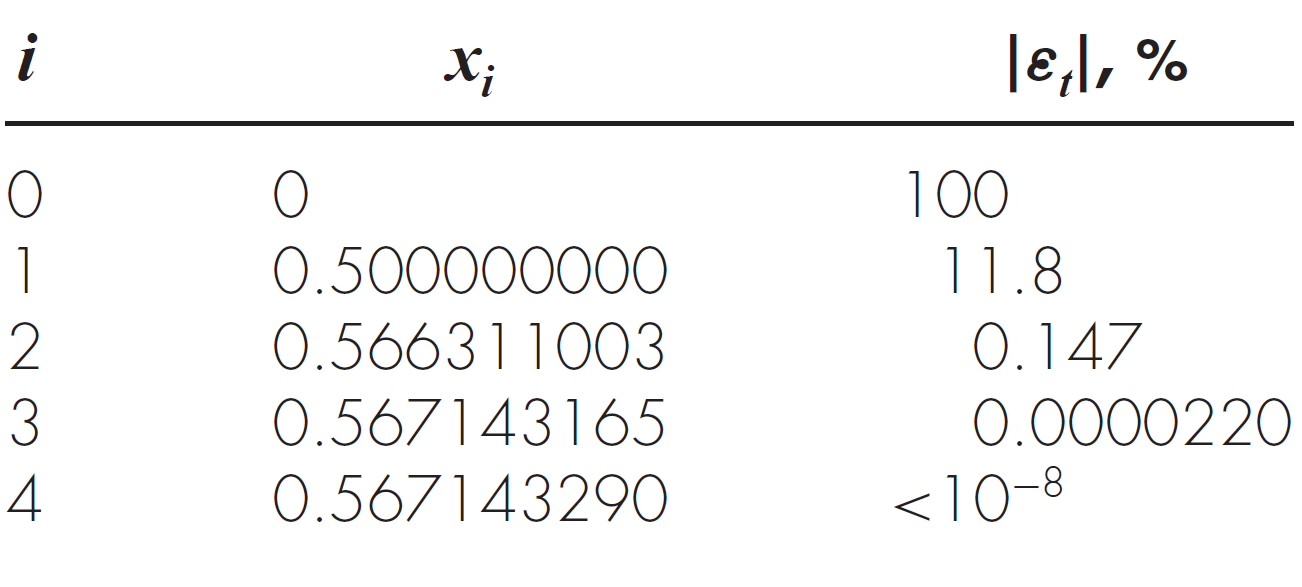
\includegraphics[width=0.4\linewidth]{./images/example_6_2_1}
    \end{figure}

    \noindent Thus, the approach rapidly converges on the true root. Notice that the true percent relative
    error at each iteration decreases much faster than it does in simple fixed-point iteration
    (compare with Example 6.1).
\end{example}

\begin{figure}[h]
    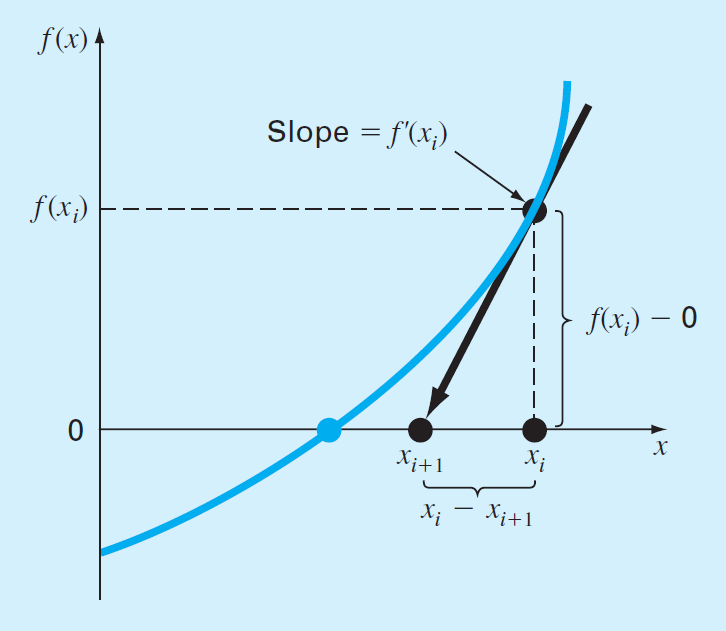
\includegraphics[width=0.55\linewidth]{./images/fig_6_4}
    \caption{Graphical depiction of the Newton-Raphson method. A tangent to the function of $x_i$ [that is,$f'(x)$] 
    is extrapolated down to the $x$ axis to provide an estimate of the root at $x_{i+1}$.}
\end{figure}

As with other root-location methods, Eq. (6.3) can be used as a termination criterion.
In addition, a theoretical analysis (Chapra and Canale, 2010) provides insight regarding the
rate of convergence as expressed by\\

$E_{t,i+1} = \dfrac{-f''(x_r)}{2f'(x_r)}E^2_{t,i}$
\hfill (6.7)\\

\noindent Thus, the error should be roughly proportional to the square of the previous error. In other
words, the number of significant figures of accuracy approximately doubles with each
iteration. This behavior is called \emph{quadratic convergence} and is one of the major reasons for
the popularity of the method.

Although the Newton-Raphson method is often very efficient, there are situations
where it performs poorly. A special case---multiple roots---is discussed elsewhere (Chapra
and Canale, 2010). However, even when dealing with simple roots, difficulties can also
arise, as in the following example.\\

\begin{example} A Slowly Converging Function with Newton-Raphson\\

    \noindent\textbf{Problem Statement.}\quad Determine the positive root of $f (x) = x^{10} - 1$ using the Newton-
    Raphson method and an initial guess of $x = 0.5$.\\

    \noindent\textbf{Solution.}\quad The Newton-Raphson formula for this case is\\
    
    $x_{i+1} = x_i - \dfrac{x^{10}_i - 1}{10x^9_i}$\\

    \noindent which can be used to compute\\

    \begin{figure}[h]
        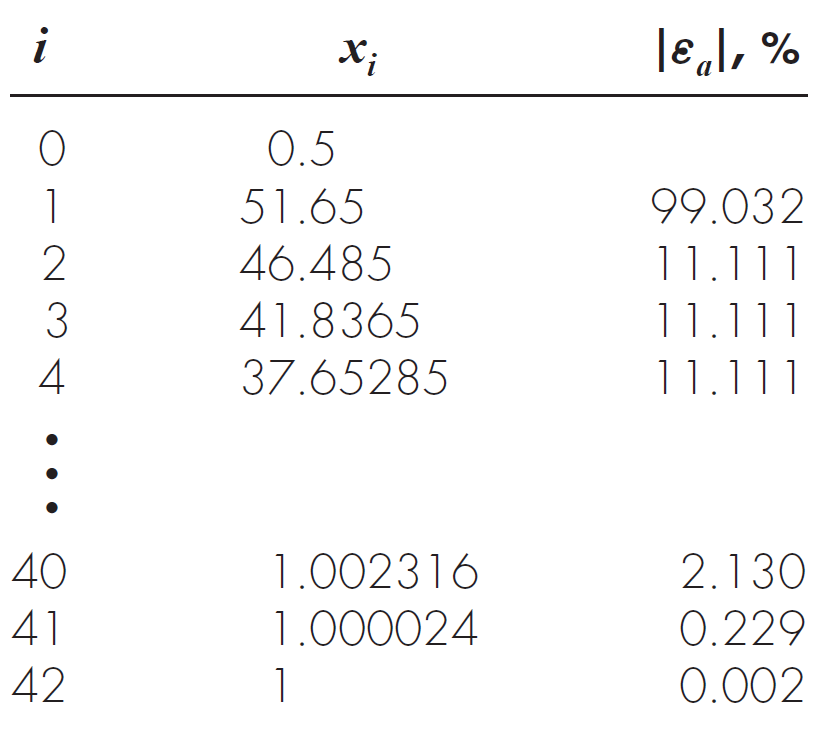
\includegraphics[width=0.3\linewidth]{./images/example_6_3_1}
    \end{figure}

    \noindent Thus, after the first poor prediction, the technique is converging on the true root of 1, but
    at a very slow rate.

    Why does this happen? As shown in Fig. 6.5, a simple plot of the first few iterations is
    helpful in providing insight. Notice how the first guess is in a region where the slope is near
    zero. Thus, the first iteration flings the solution far away from the initial guess to a new
    value ($x = 51.65$) where $f (x)$ has an extremely high value. The solution then plods along
    for over 40 iterations until converging on the root with adequate accuracy.\\

    \begin{figure}[h]
        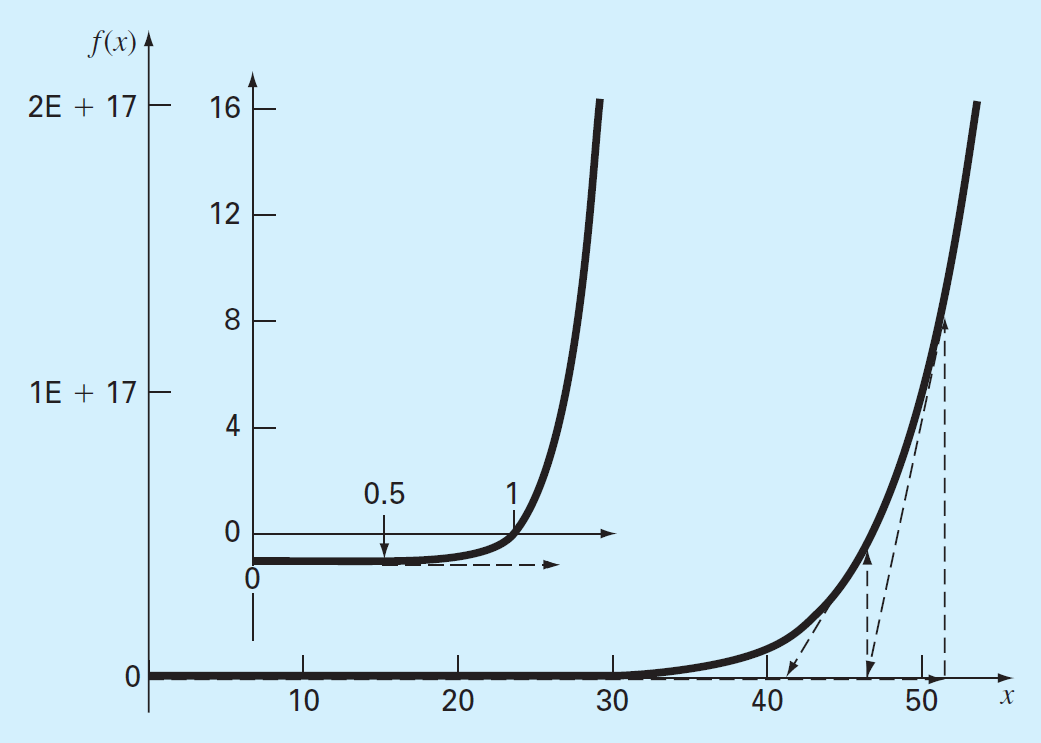
\includegraphics[width=0.6\linewidth]{./images/fig_6_5}
        \caption{Graphical depiction of the Newton-Raphson method for a case with slow convergence. The
        inset shows how a near-zero slope initially shoots the solution far from the root. Thereafter,
        the solution very slowly converges on the root.}
    \end{figure}
\end{example}

\begin{figure}[h]
    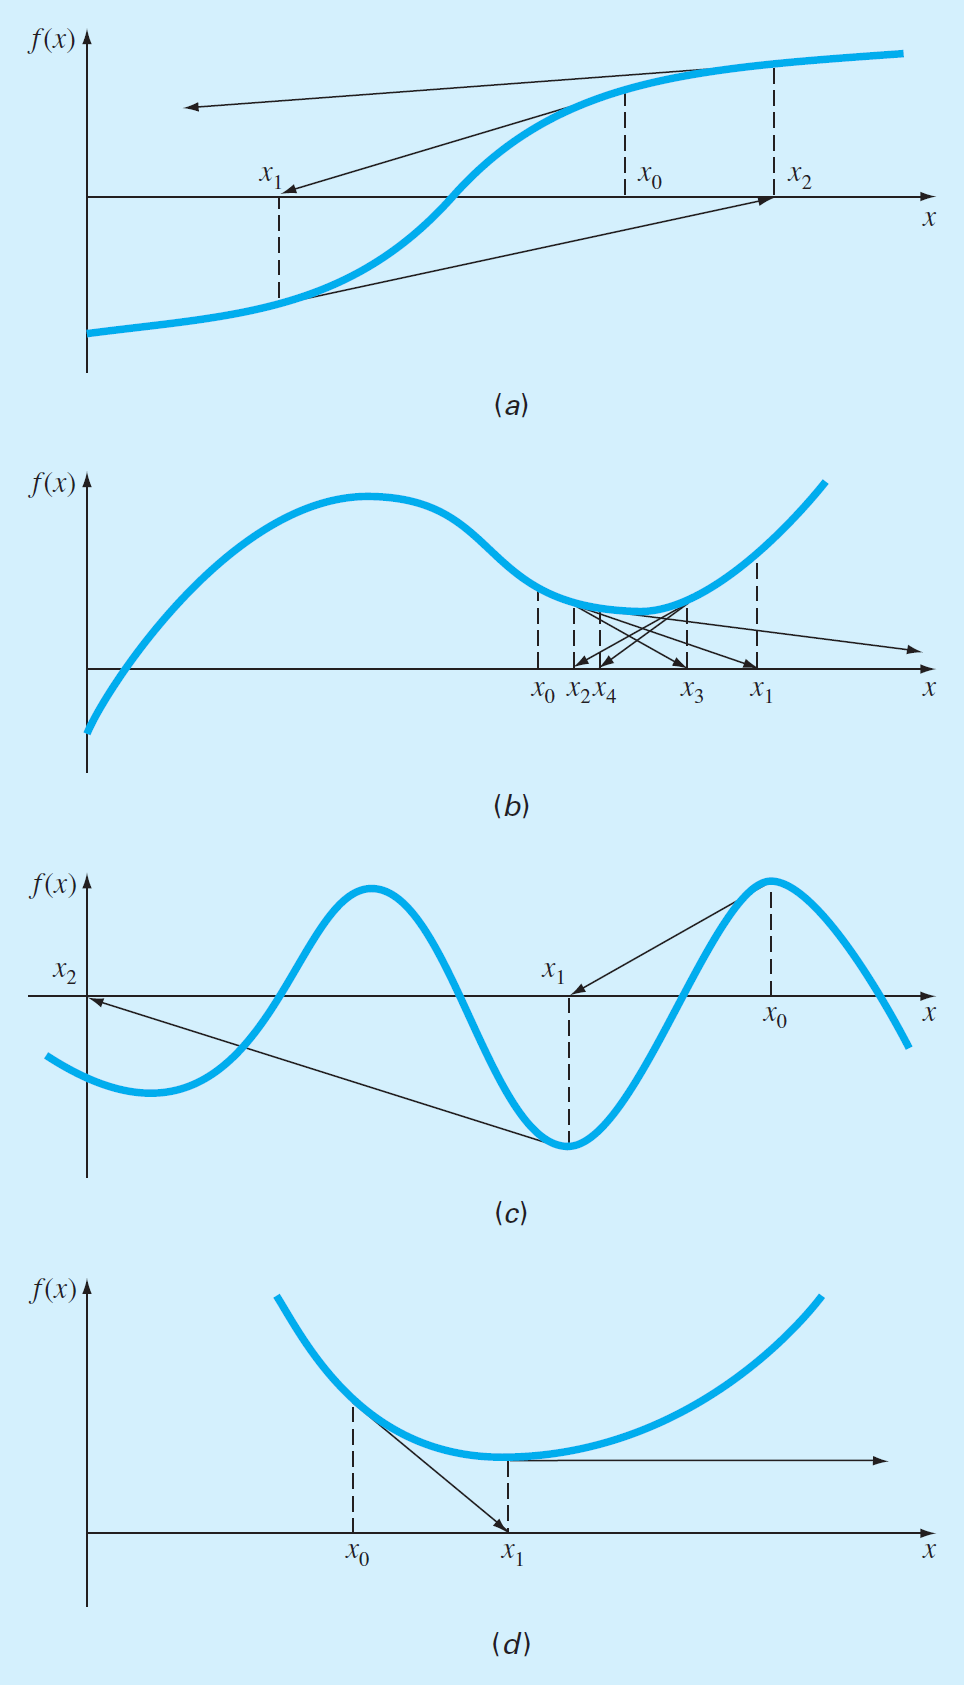
\includegraphics[width=0.5\linewidth]{./images/fig_6_6}
    \caption{Four cases where the Newton-Raphson method exhibits poor convergence.}
\end{figure}

Aside from slow convergence due to the nature of the function, other difficulties can
arise, as illustrated in Fig. 6.6. For example, Fig. 6.6a depicts the case where an inflection
point (i.e., $f'(x) = 0$) occurs in the vicinity of a root. Notice that iterations beginning at x0
progressively diverge from the root. Fig. 6.6b illustrates the tendency of the Newton-Raphson
technique to oscillate around a local maximum or minimum. Such oscillations may persist, or,
as in Fig. 6.6b, a near-zero slope is reached whereupon the solution is sent far from the area of
interest. Figure 6.6c shows how an initial guess that is close to one root can jump to a location
several roots away. This tendency to move away from the area of interest is due to the fact that
near-zero slopes are encountered. Obviously, a zero slope $[f'(x) = 0]$ is a real disaster because
it causes division by zero in the Newton-Raphson formula [Eq. (6.6)]. As in Fig. 6.6d,
it means that the solution shoots off horizontally and never hits the x axis.

Thus, there is no general convergence criterion for Newton-Raphson. Its convergence
depends on the nature of the function and on the accuracy of the initial guess. The only
remedy is to have an initial guess that is ``sufficiently'' close to the root. And for some functions,
no guess will work! Good guesses are usually predicated on knowledge of the physical
problem setting or on devices such as graphs that provide insight into the behavior of
the solution. It also suggests that good computer software should be designed to recognize
slow convergence or divergence.\\
\bigskip

\subsection{MATLAB M-file: newtraph}
\noindent An algorithm for the Newton-Raphson method can be easily developed (Fig. 6.7). Note that
the program must have access to the function (\texttt{func}) and its first derivative (\texttt{dfunc}). These
can be simply accomplished by the inclusion of user-defined functions to compute these
quantities. Alternatively, as in the algorithm in Fig. 6.7, they can be passed to the function
as arguments.

After the M-file is entered and saved, it can be invoked to solve for root. For example,
for the simple function $x^2 - 9$, the root can be determined as in\\

\texttt{>> newtraph(@(x) x\textasciicircum2-9,@(x) 2*x,5)\\
\indent ans =\\
\indent\indent 3\\}

\begin{example} Newton-Raphson Bungee Jumper Problem\\

    \noindent\textbf{Problem Statement.}\quad Use the M-file function from Fig. 6.7 to determine the mass of the
    bungee jumper with a drag coefficient of 0.25 kg/m to have a velocity of 36 m/s after 4 s of
    free fall. The acceleration of gravity is $9.81 m/s^2$.\\

    \noindent\textbf{Solution.}\quad The function to be evaluated is\\

    $f(m)=\sqrt{\dfrac{gm}{c_d}}tanh\Big(\sqrt{\dfrac{gc_d}{m}}t \Big)-v(t)$
    \hfill (E6.4.1)\\

    To apply the Newton-Raphson method, the derivative of this function must be evaluated
    with respect to the unknown, m:\\

    $\dfrac{df(m)}{dm} = \dfrac{1}{2}\sqrt{\dfrac{g}{mc_d}}tanh\Big(\sqrt{\dfrac{gc_d}{m}t} \Big)
    -\dfrac{g}{2m}t$ sech$^2\Big(\sqrt{\dfrac{gc_d}{m}}t \Big)$
    \hfill (E6.4.2)\\

    \begin{figure}[h]
        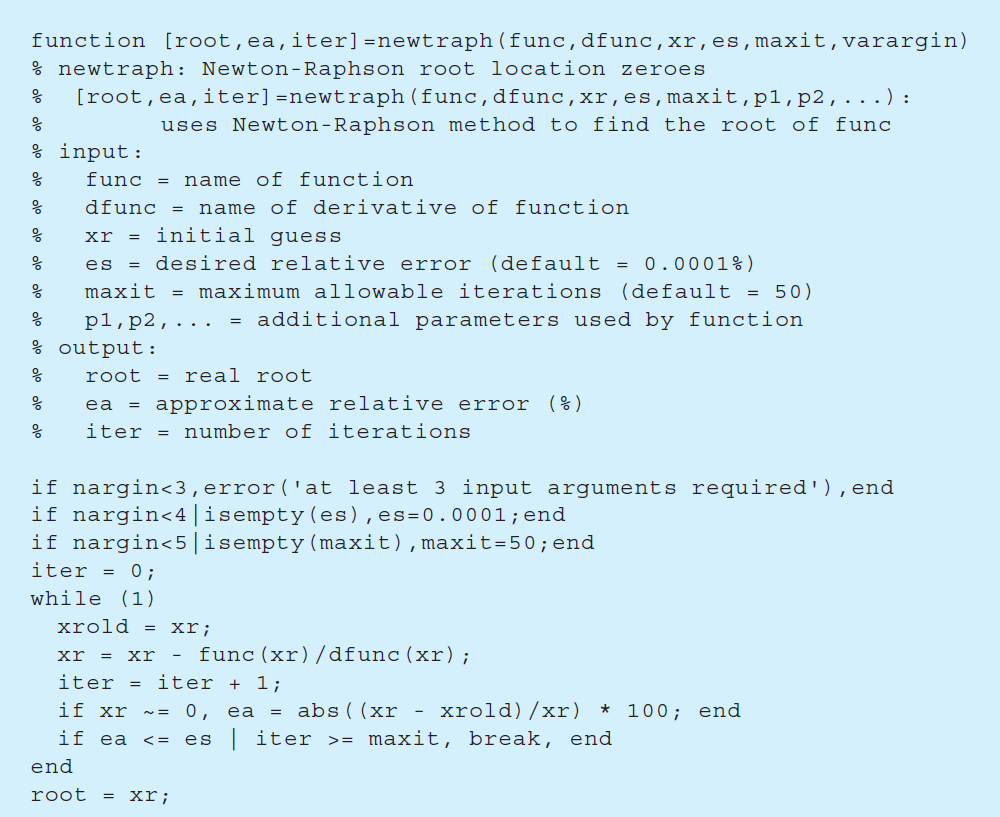
\includegraphics[width=0.8\linewidth]{./images/fig_6_7}
        \caption{An M-file to implement the Newton-Raphson method.}
    \end{figure}

    \noindent We should mention that although this derivative is not difficult to evaluate in principle, it
    involves a bit of concentration and effort to arrive at the final result.
    
    The two formulas can now be used in conjunction with the function \texttt{newtraph} to
    evaluate the root:\\

    \texttt{>> y = @m sqrt(9.81*m/0.25)*tanh(sqrt(9.81*0.25/m)*4)-36;\\
    \indent >> dy = @m 1/2*sqrt(9.81/(m*0.25))*tanh((9.81*0.25/m)\ldots\\
    \indent\indent \textasciicircum(1/2)*4)-9.81/(2*m)*sech(sqrt(9.81*0.25/m)*4)\textasciicircum2;\\
    \indent >> newtraph(y,dy,140,0.00001)\\
    \indent ans =\\
    \indent\indent 142.7376\\}
\end{example}
\bigskip

\section[SECANT METHODS]{SECANT METHODS}
\noindent As in Example 6.4, a potential problem in implementing the Newton-Raphson method is
the evaluation of the derivative. Although this is not inconvenient for polynomials and
many other functions, there are certain functions whose derivatives may be difficult or
inconvenient to evaluate. For these cases, the derivative can be approximated by a backward
finite divided difference:\\

$f'(x_i)\cong \dfrac{f(x_{i-1})-f(x_i)}{x_{i-1}-x_i}$\\

\noindent This approximation can be substituted into Eq. (6.6) to yield the following iterative
equation:\\

$x_{i+1} = x_i - \dfrac{f(x_i)(x_{i-1}-x_i)}{f(x_{i-1})-f(x_i)}$
\hfill (6.8)\\

Equation (6.8) is the formula for the \emph{secant method}. Notice that the approach requires two
initial estimates of $x$. However, because $f (x)$ is not required to change signs between the
estimates, it is not classified as a bracketing method.

Rather than using two arbitrary values to estimate the derivative, an alternative approach
involves a fractional perturbation of the independent variable to estimate $f'(x)$,\\

$f'(x_i)\cong \dfrac{f(x_i+\delta x_i)-f(x_i)}{\delta x_i}$\\

\noindent where $\delta =$ a small perturbation fraction. This approximation can be substituted into
Eq. (6.6) to yield the following iterative equation:\\

$x_{i+1} = x_i-\dfrac{\delta x_i f(x_i)}{f(x_i + \delta x_i)-f(x_i)}$
\hfill (6.9)\\

We call this the \emph{modified secant method}. As in the following example, it provides a nice
means to attain the efficiency of Newton-Raphson without having to compute derivatives.\\

\begin{example} Modified Secant Method\\

    \noindent\textbf{Problem Statement.}\quad Use the modified secant method to determine the mass of the
    bungee jumper with a drag coefficient of 0.25 kg/m to have a velocity of 36 m/s after 4 s of
    free fall. Note: The acceleration of gravity is $9.81 m/s^2$. Use an initial guess of 50 kg and a
    value of $10^{-6}$ for the perturbation fraction.\\

    \noindent\textbf{Solution.}\quad Inserting the parameters into Eq. (6.9) yields\\

    \noindent First iteration:\\

    $x_0 = 50$\hspace{28.5mm}$f(x_0) = -4.57938708$\\

    $x_0 + \delta x_0 = 50.00005$\hspace{10mm}$f(x_0+\delta x_0) = -4.579381118$\\

    $x_1 = 50-\dfrac{10^{-6}(50)(-4.57938708))}{-4.579381118 - (-4.57938708)}=
    88.39931(\left\lvert \epsilon_t \right\rvert = 38.1\%; \left\lvert \epsilon_a \right\rvert =43.4\% )$\\

    \noindent Second iteration:\\

    $x_1 = 88.39931$\hspace{20mm}$f(x_1) = -1.69220771$\\

    $x_1 + \delta x_1 = 88.39940$\hspace{11mm}$f(x_1+ \delta x_1) = -1.692203516$\\

    $x_2 = 88.39931 - \dfrac{10^{-6}(88.39931)(-1.69220771)}{-1.692203516 - (-1.69220771)} =
    124.08970(\left\lvert \epsilon_t \right\rvert = 13.1\%; \left\lvert \epsilon_a \right\rvert = 28.76\%)$\\

    \noindent The calculation can be continued to yield\\

    \begin{figure}[h]
        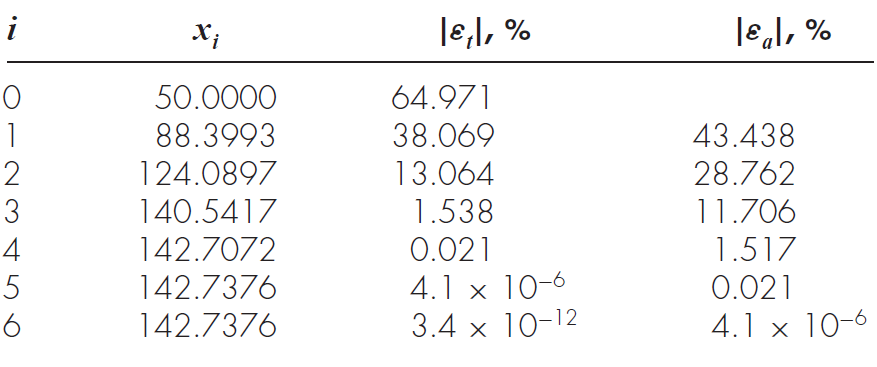
\includegraphics[width=0.4\linewidth]{./images/example_6_5_1}
    \end{figure}
    
    The choice of a proper value for $\delta$ is not automatic. If $\delta$ is too small, the method can be
    swamped by round-off error caused by subtractive cancellation in the denominator of
    Eq. (6.9). If it is too big, the technique can become inefficient and even divergent. However,
    if chosen correctly, it provides a nice alternative for cases where evaluating the
    derivative is difficult and developing two initial guesses is inconvenient.
    
    Further, in its most general sense, a univariate function is merely an entity that returns
    a single value in return for values sent to it. Perceived in this sense, functions are not
    always simple formulas like the one-line equations solved in the preceding examples in this
    chapter. For example, a function might consist of many lines of code that could take a significant
    amount of execution time to evaluate. In some cases, the function might even represent
    an independent computer program. For such cases, the secant and modified secant
    methods are valuable.\\
\end{example}
\newpage

\section[BRENT'S METHOD]{BRENT'S METHOD}
\noindent Wouldn't it be nice to have a hybrid approach that combined the reliability of bracketing
with the speed of the open methods? \emph{Brent's root-location method} is a clever algorithm that
does just that by applying a speedy open method wherever possible, but reverting to a reliable
bracketing method if necessary. The approach was developed by Richard Brent (1973)
based on an earlier algorithm of Theodorus Dekker (1969).

The bracketing technique is the trusty bisection method (Sec. 5.4), whereas two different
open methods are employed. The first is the secant method described in Sec. 6.3. As
explained next, the second is inverse quadratic interpolation.\\

\subsection{Inverse Quadratic Interpolation}
\noindent \emph{Inverse quadratic interpolation} is similar in spirit to the secant method. As in Fig. 6.8a, the
secant method is based on computing a straight line that goes through two guesses. The
intersection of this straight line with the x axis represents the new root estimate. For this
reason, it is sometimes referred to as a \emph{linear interpolation method}.

Now suppose that we had three points. In that case, we could determine a quadratic
function of $x$ that goes through the three points (Fig. 6.8b). Just as with the linear secant
method, the intersection of this parabola with the $x$ axis would represent the new root estimate.
And as illustrated in Fig. 6.8b, using a curve rather than a straight line often yields a
better estimate.

Although this would seem to represent a great improvement, the approach has a fundamental
flaw: it is possible that the parabola might not intersect the $x$ axis! Such would be
the case when the resulting parabola had complex roots. This is illustrated by the parabola,
$y = f(x)$, in Fig. 6.9.

The difficulty can be rectified by employing inverse quadratic interpolation. That is,
rather than using a parabola in x, we can fit the points with a parabola in y. This amounts to
reversing the axes and creating a ``sideways'' parabola [the curve, $x = f(y)$, in Fig. 6.9].

If the three points are designated as $(x_{i-2}, y_{i-2})$, $(x_{i-1}, y_{i-1})$, and $(x_i, y_i)$, a quadratic
function of y that passes through the points can be generated as\\

$g(y) = \dfrac{(y-y_{i-1})(y-y_i)}{(y_{i-2}-y_{i-1})(y_{i-2}-y_i)}x_{i-2}+
\dfrac{(y-y_{i-2})(y-y_i)}{(y_{i-1}-y_{i-2})(y_{i-1}-y_i)}x_{i-1}+
\dfrac{(y-y_{i-2})(y-y_{i-1})}{(y_{i}-y_{i-2})(y_{i}-y_{i-1})}x_{i}$
\hfill (6.10)\\
\bigskip

\begin{figure}[h]
    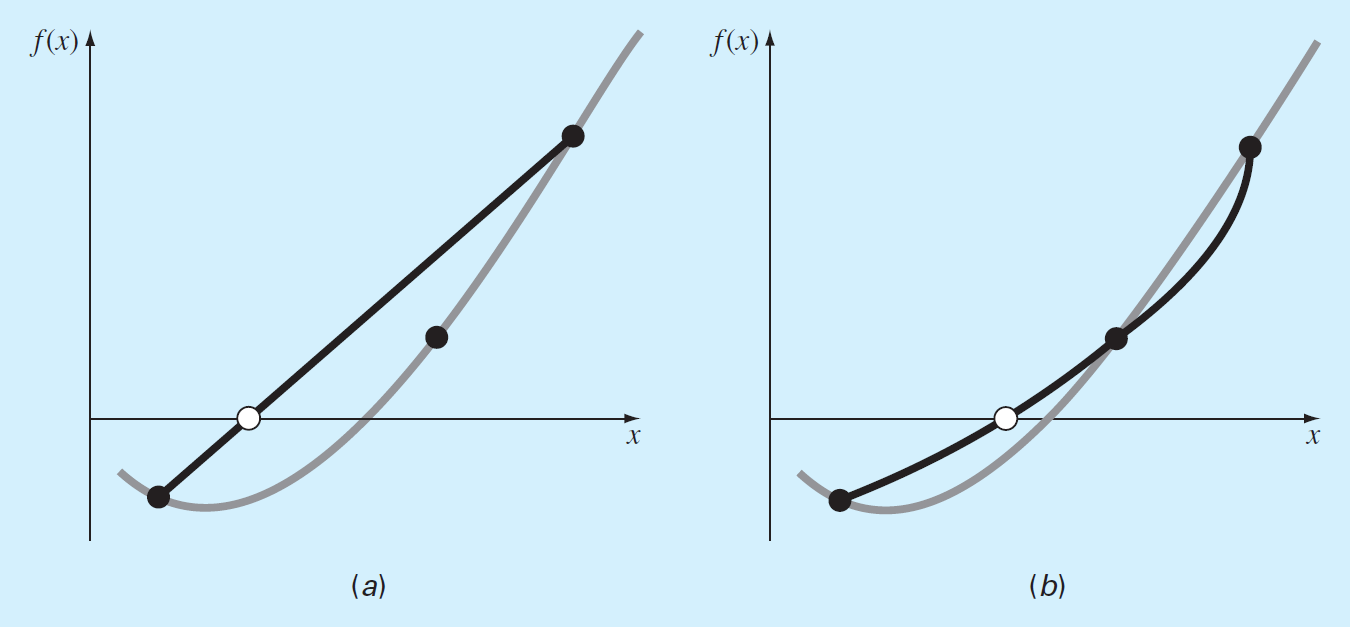
\includegraphics[width=0.8\linewidth]{./images/fig_6_8}
    \caption{Comparison of (a) the secant method and (b) inverse quadratic interpolation. Note that the
    approach in (b) is called ``inverse'' because the quadratic function is written in y rather than in $x$.}
\end{figure}

\begin{figure}[h]
    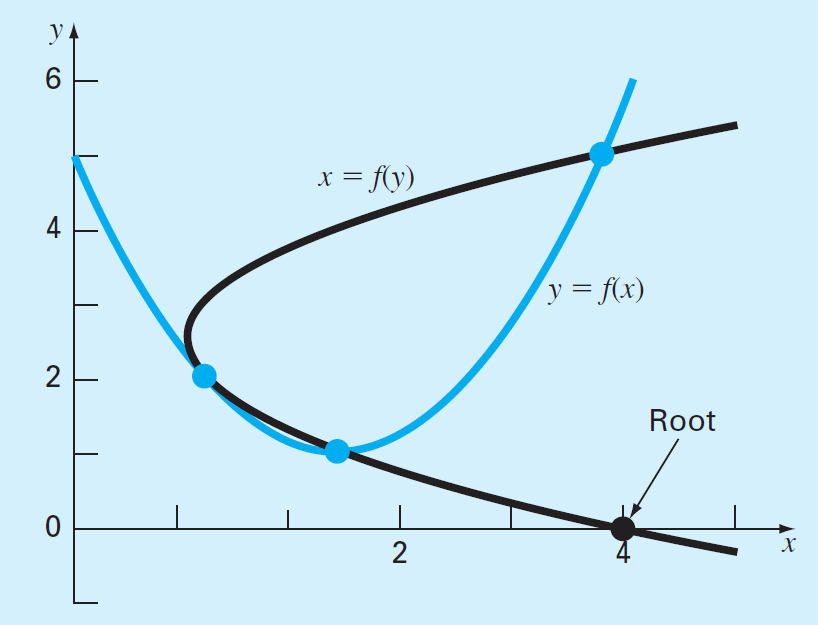
\includegraphics[width=0.5\linewidth]{./images/fig_6_9}
    \caption{Two parabolas fit to three points. The parabola written as a function of $x, y = f(x)$, has complex
    roots and hence does not intersect the $x$ axis. In contrast, if the variables are reversed, and the
    parabola developed as $x = f (y)$, the function does intersect the $x$ axis.}
\end{figure}
\bigskip

\noindent As we will learn in Sec. 18.2, this form is called a \emph{Lagrange polynomial}. The root, $x_{i+1}$, corresponds
to $y = 0$, which when substituted into Eq. (6.10) yields\\

$x_{i+1}= \dfrac{y_{i-1}y_i}{(y_{i-2} - y_{i-1})(y_{i-2} - y_i)}x_{i-2}+
\dfrac{y_{i-2}y_i}{(y_{i-1} - y_{i-2})(y_{i-1} - y_i)}x_{i-1}+
\dfrac{y_{i-2}y_{i-1}}{(y_{i} - y_{i-2})(y_{i} - y_{i-1})}x_{i}$
\hfill (6.11)\\
\bigskip

\noindent As shown in Fig. 6.9, such a ``sideways'' parabola always intersects the $x$ axis.
\newpage

\begin{example} Inverse Quadratic Interpolation\\

    \noindent\textbf{Problem Statement. }\quad Develop quadratic equations in both $x$ and $y$ for the data points
    depicted in Fig. 6.9: $(1, 2)$, $(2, 1)$, and $(4, 5)$. For the first, $y = f(x)$, employ the quadratic
    formula to illustrate that the roots are complex. For the latter, $x = g(y)$, use inverse quadratic
    interpolation (Eq. 6.11) to determine the root estimate.\\

    \noindent\textbf{Solution.}\quad By reversing the $x$'s and $y$'s, Eq. (6.10) can be used to generate a quadratic in $x$ as\\

    $f(x) = \dfrac{(x-2)(x-4)}{(1-2)(1-4)}2 + \dfrac{(x-1)(x-4)}{(2-1)(2-4)}1 +
    \dfrac{(x-1)(x-2)}{(4-1)(4-2)}5$\\

    \noindent or collecting terms\\

    $f(x)= x^2 - 4x + 5$\\

    \noindent This equation was used to generate the parabola, $y = f(x)$, in Fig. 6.9. The quadratic formula
    can be used to determine that the roots for this case are complex,\\

    $x = \dfrac{4\pm \sqrt{(-4)^2 - 4(1)(5)}}{2} = 2\pm i$\\

    \noindent Equation (6.10) can be used to generate the quadratic in $y$ as\\

    $g(y) = \dfrac{(y-1)(y-5)}{(2-1)(2-5)}1 + \dfrac{(y-2)(y-5)}{(1-2)(1-5)}2 +
    \dfrac{(y-2)(y-1)}{(5-2)(5-1)}4$\\

    \noindent or collecting terms:\\

    $g(y) = 0.5x^2-2.5x+4$\\

    \noindent Finally, Eq. (6.11) can be used to determine the root as\\

    $x_{i+1} = \dfrac{-1(-5)}{(2-1)(2-5)}1 + \dfrac{-2(-5)}{(1-2)(1-5)}2 +
    \dfrac{-2(-1)}{(5-2)(5-1)}4 = 4$\\    
\end{example}

Before proceeding to Brent's algorithm, we need to mention one more case where
inverse quadratic interpolation does not work. If the three $y$ values are not distinct (i.e.,
$y_{i-2} = y_{i-1}$ or $y_{i-1} = y_i$), an inverse quadratic function does not exist. So this is where the
secant method comes into play. If we arrive at a situation where the $y$ values are not distinct,
we can always revert to the less efficient secant method to generate a root using two of
the points. If $y_{i-2} = y_{i-1}$, we use the secant method with $x_{i-1}$ and $x_i$. If $y_{i-1} = y_i$, we use $x_{i-2}$
and $x_{i-1}$.
\newpage

\section{Brent's Method Algorithm}
\noindent The general idea behind the \emph{Brent's root-finding method} is whenever possible to use one of
the quick open methods. In the event that these generate an unacceptable result (i.e., a root
estimate that falls outside the bracket), the algorithm reverts to the more conservative
bisection method. Although bisection may be slower, it generates an estimate guaranteed to
fall within the bracket. This process is then repeated until the root is located to within an
acceptable tolerance. As might be expected, bisection typically dominates at first but as the
root is approached, the technique shifts to the faster open methods.

Figure 6.10 presents a function based on a MATLAB M-file developed by Cleve
Moler (2004). It represents a stripped down version of the \texttt{fzero} function which is the professional
root-location function employed in MATLAB. For that reason, we call the
simplified version: \texttt{fzerosimp}. Note that it requires another function \texttt{f} that holds the
equation for which the root is being evaluated.

The \texttt{fzerosimp} function is passed two initial guesses that must bracket the root.
Then, the three variables defining the search interval \texttt{(a,b,c)} are initialized, and \texttt{f} is evaluated
at the endpoints.\\

\begin{figure}[h]
    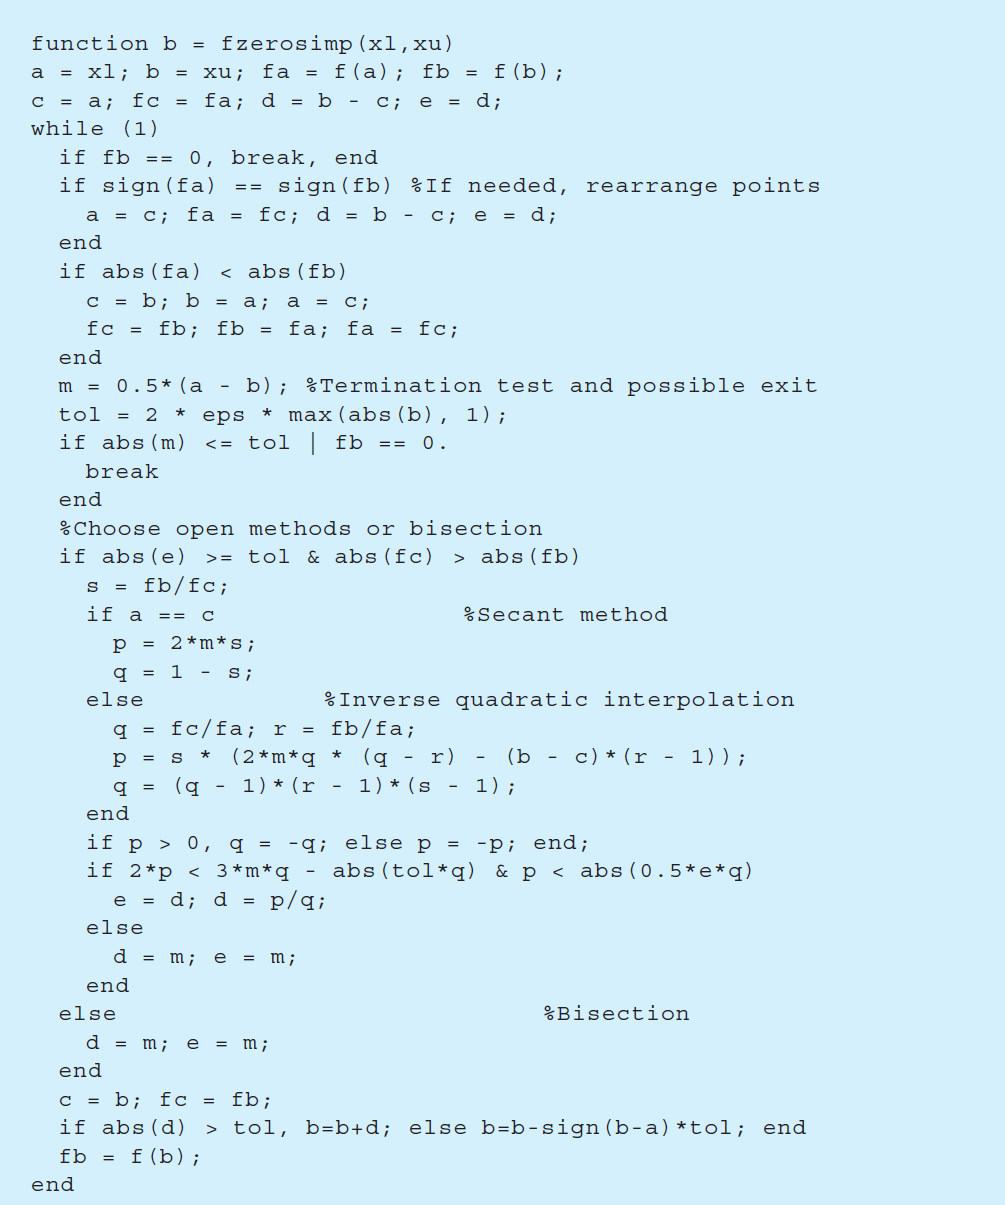
\includegraphics[width=0.8\linewidth]{./images/fig_6_10}
    \caption{Function for Brent's root-finding algorithm based on a MATLAB M-file developed by Cleve Moler
    (2005).}
\end{figure}

A main loop is then implemented. If necessary, the three points are rearranged to satisfy
the conditions required for the algorithm to work effectively. At this point, if the stopping
criteria are met, the loop is terminated. Otherwise, a decision structure chooses among the
three methods and checks whether the outcome is acceptable. Afinal section then evaluates
\texttt{f} at the new point and the loop is repeated. Once the stopping criteria are met, the loop
terminates and the final root estimate is returned.\\

\section[MATLAB FUNCTION: fzero]{MATLAB FUNCTION: fzero}
\noindent The \texttt{fzero} function is designed to find the real root of a single equation. A simple representation
of its syntax is\\

\texttt{fzero(function, x0)}\\

\noindent where \texttt{function} is the name of the function being evaluated, and \texttt{x0} is the initial guess.
Note that two guesses that bracket the root can be passed as a vector:\\

\texttt{fzero(function,[x0 x1])}\\

\noindent where x0 and x1 are guesses that bracket a sign change.\\

\noindent Here is a simple MATLAB session that solves for the root of a simple quadratic: $x^2 - 9$.
Clearly two roots exist at -3 and 3. To find the negative root:\\

\texttt{>> x = fzero(@(x) x\textasciicircum2-9,-4)\\
\indent x =\\
\indent\indent 3}\\

\noindent If we want to find the positive root, use a guess that is near it:\\

\texttt{>> x = fzero(@(x) x\textasciicircum2-9,4\\)
\indent x =\\
\indent\indent 3}\\

\noindent If we put in an initial guess of zero, it finds the negative root:\\

\texttt{>> x = fzero(@(x) x\textasciicircum2-9,0)\\
\indent x =\\
\indent\indent -3}\\

\noindent If we wanted to ensure that we found the positive root, we could enter two guesses as in\\

\texttt{>> x = fzero(@(x) x\textasciicircum2-9,[0 4])\\
\indent x =\\
\indent\indent 3}\\

\noindent Also, if a sign change does not occur between the two guesses, an error message is displayed\\

\texttt{>> x = fzero(@(x) x\textasciicircum2-9,[-4 4])\\
\indent ??? Error using ==> fzero\\
\indent The function values at the interval endpoints must differ in sign.}\\

\noindent The \texttt{fzero} function works as follows. If a single initial guess is passed, it first performs
a search to identify a sign change. This search differs from the incremental search described
in Section 5.3.1, in that the search starts at the single initial guess and then takes increasingly
bigger steps in both the positive and negative directions until a sign change is detected.

Thereafter, the fast methods (secant and inverse quadratic interpolation) are used unless
an unacceptable result occurs (e.g., the root estimate falls outside the bracket). If an
unacceptable result happens, bisection is implemented until an acceptable root is obtained
with one of the fast methods. As might be expected, bisection typically dominates at first
but as the root is approached, the technique shifts to the faster methods.

A more complete representation of the fzero syntax can be written as\\

\texttt{[x,fx] = fzero(function,x0,options,p1,p2,...)}\\

\noindent where \texttt{[x,fx]} = a vector containing the root \texttt{x} and the function evaluated at the root \texttt{fx},
\texttt{options} is a data structure created by the \texttt{optimset} function, and \texttt{p1, p2}... are any
parameters that the function requires. Note that if you desire to pass in parameters but not
use the \texttt{options}, pass an empty vector [] in its place.

The \texttt{optimset} function has the syntax\\

\texttt{options = optimset('par1',val1,'par2',val2,...)}\\

\noindent where the parameter \texttt{$par_i$} has the value \texttt{$val_i$}. A complete listing of all the possible parameters
can be obtained by merely entering \texttt{optimset} at the command prompt. The parameters
that are commonly used with the \texttt{fzero} function are\\

\texttt{display:} When set to \texttt{'iter'} displays a detailed record of all the iterations.\\
\texttt{tolx:} A positive scalar that sets a termination tolerance on \texttt{x}.

\begin{example} The \texttt{fzero} and \texttt{optimset} Functions\\

    \noindent\textbf{Problem Statement.}\quad Recall that in Example 6.3, we found the positive root of $f (x) = x^{10} - 1$ 
    using the Newton-Raphson method with an initial guess of 0.5. Solve the same problem with \texttt{optimset} and \texttt{fzero}.\\

    \noindent\textbf{Solution.}\quad An interactive MATLAB session can be implemented as follows:\\

    \texttt{>> options = optimset('display','iter');\\
    \indent >> [x,fx] = fzero(@(x) x\textasciicircum10-1,0.5,options)\\}

    %\texttt{\begin{tabular}{c c c c}
    %    Func-count & x & f(x) & Procedure\\
    %    1  &  0.5      & -0.999023 & initial\\
    %    2  &  0.485858 & -0.999267 & search\\
    %    3  &  0.514142 & -0.998709 & search\\
    %    4  &  0.48     & -0.999351 & search\\
    %    5  &  0.52     & -0.998554 & search\\
    %    6  &  0.471716 & -0.999454 & search\\
    %    $\bullet$  &  & & \\
    %    $\bullet$  &  & & \\
    %    $\bullet$  &  & & \\
    %    23 &  0.952548 & -0.385007 & search\\
    %    24 &  -0.14    & -1        & search\\
    %    25 &  1.14     &  2.70722  & search\\
    %\end{tabular}}
    %\bigskip

    %\texttt{\noindent Looking for a zero in the interval [-0.14, 1.14]}\\

    %\texttt{\begin{tabular}{c c c c}
    %    26 & 0.205272 & -1 & interpolation\\
    %    27 & 0.672636 & -0.981042 & bisection\\
    %    28 & 0.906318 & -0.626056 & bisection\\
    %    29 & 1.02316  & 0.257278 & bisection\\
    %    30 & 0.989128 & -0.103551 & interpolation\\
    %    31 & 0.998894 & -0.0110017 & interpolation\\
    %    32 & 1.00001  & 7.68385e-005 & interpolation\\
    %    33 & 1        & -3.83061e-007 & interpolation\\
    %    34 & 1        & -1.3245e-011 & interpolation\\
    %    35 & 1        & 0 & interpolation\\
    %\end{tabular}}
    
    \begin{figure}[h]
        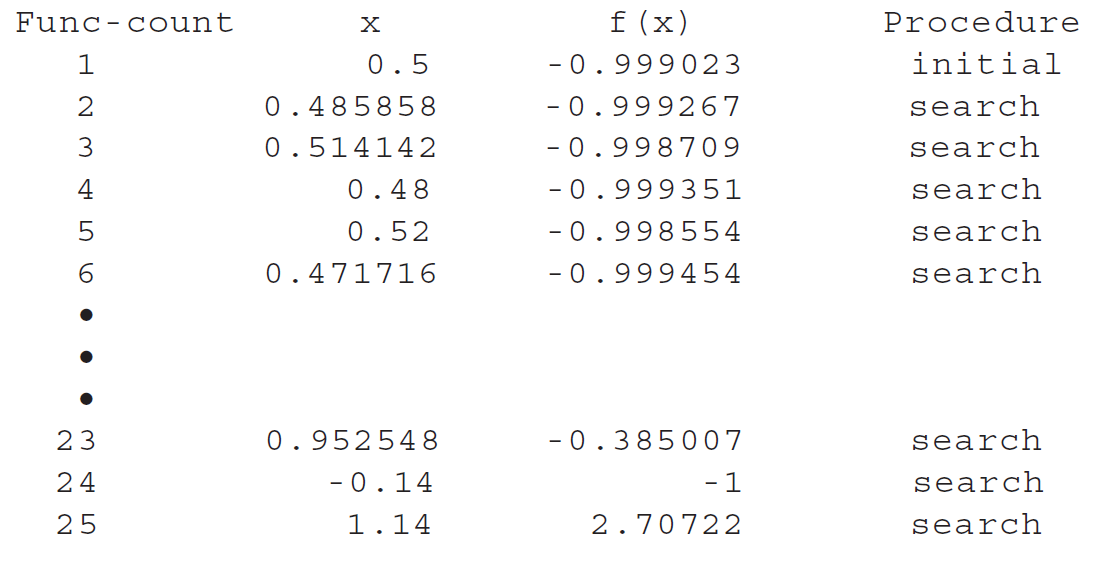
\includegraphics[width=0.6\linewidth]{./images/example_6_7_1}
    \end{figure}

    \texttt{Looking for a zero in the interval [-0.14, 1.14]}\\

    \begin{figure}[h]
        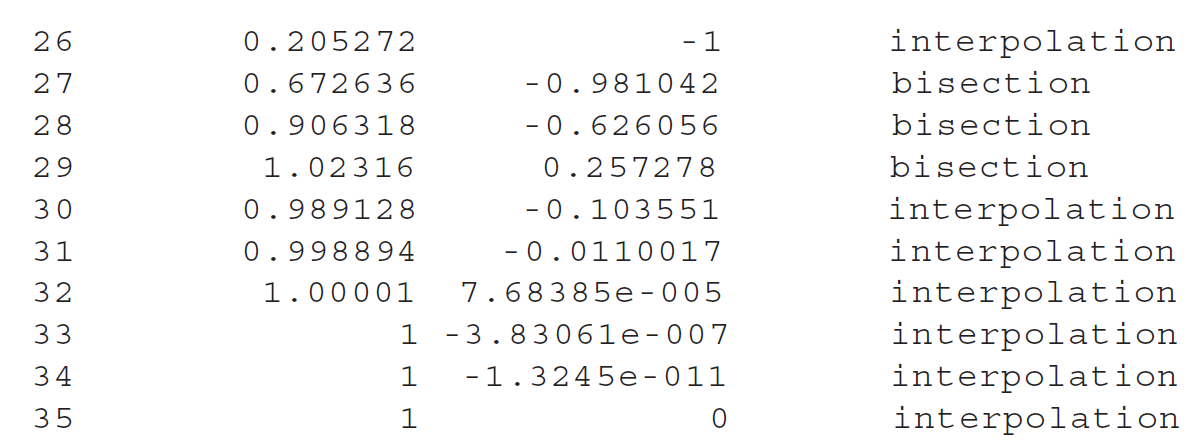
\includegraphics[width=0.6\linewidth]{./images/example_6_7_2}
    \end{figure}

    \texttt{Zero found in the interval: [-0.14, 1.14].\\
    \indent x =\\
    \indent\indent 1\\
    \indent fx =\\
    \indent\indent 0\\}

    Thus, after 25 iterations of searching, \texttt{fzero} finds a sign change. It then uses interpolation
    and bisection until it gets close enough to the root so that interpolation takes over and
    rapidly converges on the root.
    Suppose that we would like to use a less stringent tolerance. We can use the \texttt{optimset}
    function to set a low maximum tolerance and a less accurate estimate of the root results:\\

    \texttt{>> options = optimset ('tolx', 1e-3);\\
    \indent >> [x,fx] = fzero(@(x) x\textasciicircum10-1,0.5,options)\\
    \indent x =\\
    \indent\indent 1.0009\\
    \indent fx =\\
    \indent\indent 0.0090\\}
\end{example}
\bigskip

\section[POLYNOMIALS]{POLYNOMIALS}

\end{document}